\section{Bias correction}
\label{sec:bias}

The observed binary fraction is a lower limit on the true binary fraction,
since spectroscopic surveys are biased against detecting systems with long
orbital periods, low inclinations, or low mass ratios. Following the
methodology of \citet{Dsilva2023}, we employ a Monte-Carlo simulation to
constrain the intrinsic binary fraction $f_\mathrm{bin}$ and the
orbital-period distribution exponent $\pi$.

\subsection{Simulation framework}
\label{sec:sim_framework}

For each point on a two-dimensional grid in $(f_\mathrm{bin}, \pi)$, we
generate \Nsim synthetic stellar systems as follows:

\begin{enumerate}
\item Each system is assigned as binary with probability $f_\mathrm{bin}$,
  or single otherwise.

\item For binary systems, orbital parameters are drawn from the following
  distributions:
  \begin{itemize}
  \item \textbf{Period:} $p(\log P) \propto (\log P)^{\pi}$, with
    $\log P \in [0.15, 5.0]$\,days.
  \item \textbf{Eccentricity:} uniform on $[0, e_\mathrm{max}]$ with
    $e_\mathrm{max} = 0.9$.
  \item \textbf{Mass ratio:} $q = M_2/M_1$ uniform on $[0.1, 2.0]$.
  \item \textbf{Inclination:} $p(i) \propto \sin i$, $i \in [0, \pi/2]$
    (isotropic orientations).
  \item \textbf{Primary mass:} $M_1 = 10$\,\Msun (fixed) or drawn
    uniformly from $[10, 20]$\,\Msun.
  \end{itemize}

\item The radial-velocity semi-amplitude $K_1$ is computed from Kepler's
  third law:
  \begin{equation}
  K_1 = \left(\frac{2\pi G}{P}\right)^{1/3}
        \frac{M_2 \sin i}{(M_1 + M_2)^{2/3}}
        \frac{1}{\sqrt{1 - e^2}}.
  \label{eq:K1}
  \end{equation}

\item Radial-velocity curves are generated by solving Kepler's equation
  numerically, sampling at the actual observation epochs (MJD timestamps)
  of each of the \Nstars target stars. Crucially, the simulation is
  \emph{cadence-aware}: each simulated set contains exactly one star per
  real target, sampled at that target's actual MJD epochs. This faithfully
  reproduces the observational sampling and per-star cadence limitations.
  $N_\mathrm{sets}$ such sets are generated (typically $N_\mathrm{sets} =
  500$--3000), and the simulated CDF is constructed from the median binary
  fraction in each $\Delta\mathrm{RV}$ bin across all realisations.

\item Observational noise is added to \emph{both} single and binary
  stars. For single stars, the noise is drawn from a distribution with
  characteristic scale $\sigma_\mathrm{single}$ (intrinsic wind
  variability). For binary stars, per-epoch measurement noise is drawn
  from a separate error model distribution, ensuring that face-on or
  long-period binaries with $\Delta\mathrm{RV} \approx 0$ still exhibit
  realistic scatter. This prevents the likelihood score from favouring
  $f_\mathrm{bin} = 1$ (where noise-free face-on binaries mimic singles
  at zero cost). Both error model distributions may be fitted to the
  observed per-epoch RV uncertainties.
\end{enumerate}

\subsection{Comparison to observations}
\label{sec:likelihood_test}

For each grid point, we compute the peak-to-peak
$\Delta\mathrm{RV}_\mathrm{max}$ of each simulated star. A simulated star
is classified as a detected binary only if it satisfies the same two
criteria applied to the real data (Sect.~\ref{sec:criteria}): (1)
$\Delta\mathrm{RV}_\mathrm{max} > T$ for a given threshold $T$, and (2)
$\Delta\mathrm{RV} - \sigthresh\,\sigma_\mathrm{p2p} > 0$, where
$\sigma_\mathrm{p2p} = \sqrt{\sigma_\mathrm{max}^2 +
\sigma_\mathrm{min}^2}$ is the combined measurement uncertainty at the
epochs of maximum and minimum RV. This significance criterion prevents
noise-dominated detections at low thresholds and ensures consistency
between the simulated and observed binary fraction curves. The three known
Bartzakos binaries are added to the observed count at all thresholds
(denominator $N = 28$).

To compare the simulated and observed $\Delta\mathrm{RV}$ distributions,
we adopt the multinomial likelihood scheme of \citet{Dsilva2023}
(Sect.~4.2). The $\Delta\mathrm{RV}$ axis is partitioned into coarse
intervals with default edges $\{0,\,\drvthresh,\,250,\,650,\,\infty\}$\,\kms,
where the lowest edge coincides with the binary detection threshold so that
the first bin isolates non-detections and the remaining bins resolve the
high-amplitude tail. Let $n_i$ denote the observed count in bin $i$ and
$p_i$ the corresponding fraction predicted by the Monte-Carlo simulation
at a given grid point; the likelihood of the observed counts under the
simulated model is
\begin{equation}
\mathcal{L}(\mathbf{n}\,|\,\mathbf{p}) =
\frac{N!}{\prod_i n_i!}\,\prod_i p_i^{\,n_i},
\label{eq:multinomial}
\end{equation}
with $N = \Ntotal$. The best-fit model is the grid point that maximises
$\ln\mathcal{L}$.

\begin{figure}
\centering
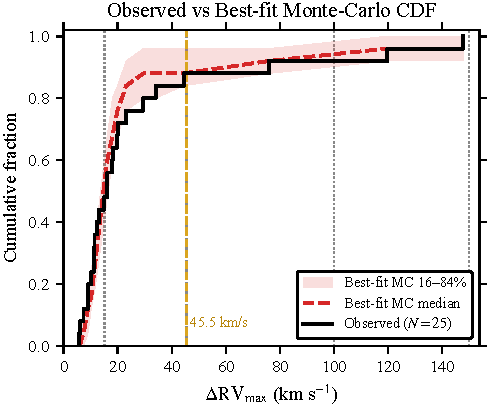
\includegraphics[width=\columnwidth]{plots/cdf_obs_vs_sim.pdf}
\caption{Cumulative $\Delta\mathrm{RV}_{\max}$ distribution: observations
  (black solid step) vs.\ Monte-Carlo simulation at the best-fit grid
  point (red dashed; the 16--84\% percentile band of the simulation is
  shaded). The vertical dashed lines mark the multinomial bin edges
  (Eq.~\ref{eq:multinomial}). \emph{Preliminary snapshot}: the
  bias-correction grid is still being tuned and the values shown
  correspond to a representative grid configuration with
  $N_\mathrm{sim} = 1000$ realisations.}
\label{fig:cdf_obs_vs_sim}
\end{figure}

\subsection{Grid search and results}
\label{sec:grid_results}

The grid spans $f_\mathrm{bin} \in [0.3, 1.0]$ with step 0.005--0.01, and
$\pi \in [-3, +1]$. The search is parallelised across
$N_\mathrm{cores} - 1$ CPU cores.

The best-fit parameters are $f_\mathrm{bin} =
{\fbincorr}^{+\fbinerrup}_{-\fbinerrdn}$ and $\pi =
{\pibestfit}^{+\pierrup}_{-\pierrdn}$, where the uncertainties represent
68\% highest-density intervals (HDI68) from the marginalised
log-likelihood.

\begin{figure}
\centering
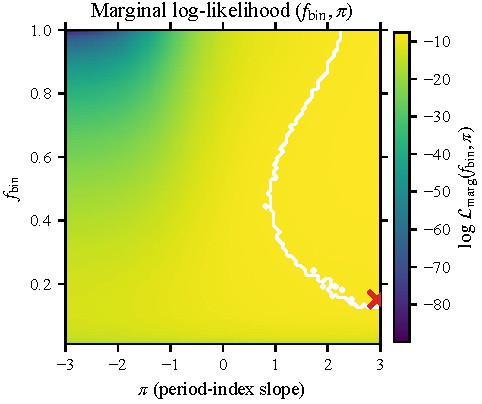
\includegraphics[width=\columnwidth]{plots/fbin_pi_heatmap.pdf}
\caption{Marginalised log-likelihood over $(f_\mathrm{bin}, \pi)$ for the
  Dsilva power-law period model. The cross marks the joint argmax; the
  white contour encloses the 68\% highest-density interval (HDI68). The
  likelihood is marginalised over the nuisance parameters
  $\sigma_\mathrm{single}$ and $\log P_\mathrm{max}$. \emph{Preliminary
  snapshot}: bias-correction grid not yet converged.}
\label{fig:fbin_pi_heatmap}
\end{figure}

\begin{figure}
\centering
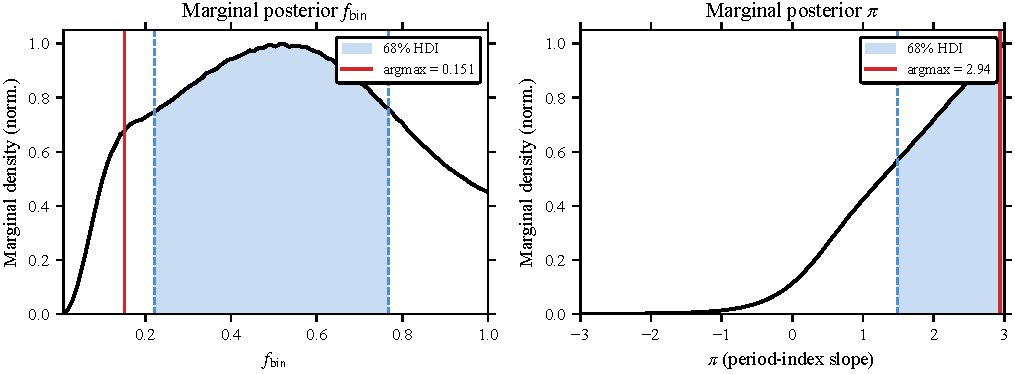
\includegraphics[width=\columnwidth]{plots/fbin_pi_marginals.pdf}
\caption{One-dimensional marginal posteriors of (\textit{left}) the
  binary fraction $f_\mathrm{bin}$ and (\textit{right}) the
  period-distribution exponent $\pi$, derived from the Dsilva grid of
  Fig.~\ref{fig:fbin_pi_heatmap}. The solid vertical lines mark the
  joint argmax; the dashed lines and shaded regions mark the 68\% HDI
  bounds. \emph{Preliminary snapshot}.}
\label{fig:fbin_pi_marginals}
\end{figure}

\begin{figure}
\centering
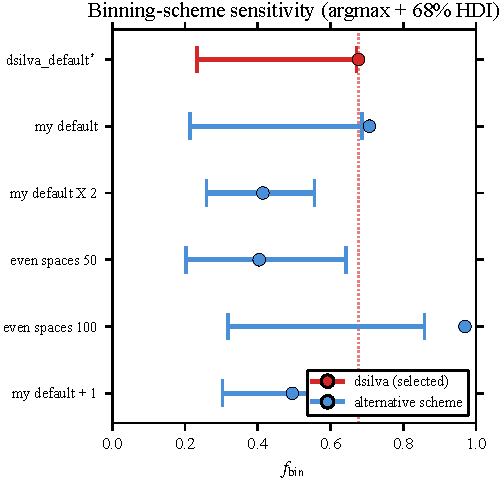
\includegraphics[width=\columnwidth]{plots/bin_sensitivity.pdf}
\caption{Bin-choice sensitivity of the inferred binary fraction. For each
  multinomial-bin scheme tested, the marker is the argmax $f_\mathrm{bin}$
  and the horizontal bar covers the 68\% HDI. The default scheme of
  \citet{Dsilva2023} ($\{0,\drvthresh,250,650,\infty\}$\,\kms) is
  highlighted in red; alternative schemes vary in number of bins, edge
  placement, and edge spacing. The envelope across schemes is reported
  as a methodological-robustness statement alongside the headline value.}
\label{fig:bin_sensitivity}
\end{figure}

